
\noindent\begin{minipage}{\textwidth}
    \begin{table}[H]
        \centering
        \caption{Hiperparâmetros e Resultados do Melhor Modelo - inception\_v10\_BR\_opt\_aug}
        \vspace{0.2cm}
        \resizebox{\textwidth}{!}{%
            \begin{tabular}{ll | lrrr}
                \hline
                \multicolumn{2}{c|}{\textbf{Hiperparâmetros}} & \multicolumn{4}{c}{\textbf{Métricas por Classe}} \\ \hline
                \textbf{Parâmetro} & \textbf{Valor} & \textbf{Classe} & \textbf{Precisão} & \textbf{Recall} & \textbf{F1-Score} \\ \hline
    Agendador (Patience) & 5 & 31.2 & 0.4641 & 0.4955 & 0.4793 \\ 
Agendador de LR & ReduceLROnPlateau & 31.3 & 0.3500 & 0.3351 & 0.3424 \\ 
Architecture & inception\_v3 & 31.4 & 0.3757 & 0.3114 & 0.3405 \\ 
Augmentation (Método) & None & 32.3 & 0.4716 & 0.4392 & 0.4548 \\ 
Batch Size & 32 & 32.4 & 0.2222 & 0.2778 & 0.2469 \\ 
Decaimento de Peso (WD) & 0.0001 & 33.3 & 0.3720 & 0.4306 & 0.3991 \\ 
Dropout & 0.4422 & 41.4 & 0.3200 & 0.1702 & 0.2222 \\ 
Função de Perda & CrossEntropyLoss & 41.5 & 0.4464 & 0.5814 & 0.5051 \\ 
Hidden Units & 1024 & 42.4 & 0.2838 & 0.3443 & 0.3111 \\ 
Label Smoothing & 0.1000 & 44.4 & 0.4000 & 0.3750 & 0.3871 \\ 
\cline{3-6} 
Otimizador & AdamW & \textbf{Média (Macro)} & 0.4029 & 0.3916 & 0.3936 \\ 
Taxa de Aprendizado (LR) & 5.72e-04 & \textbf{MCC} & \multicolumn{3}{c}{0.3188} \\ 
Unfreeze Layers & 6 &  & & &  \\ 
            \hline
            \end{tabular}%
        }
    \end{table}

    \begin{figure}[H]
        \centering
        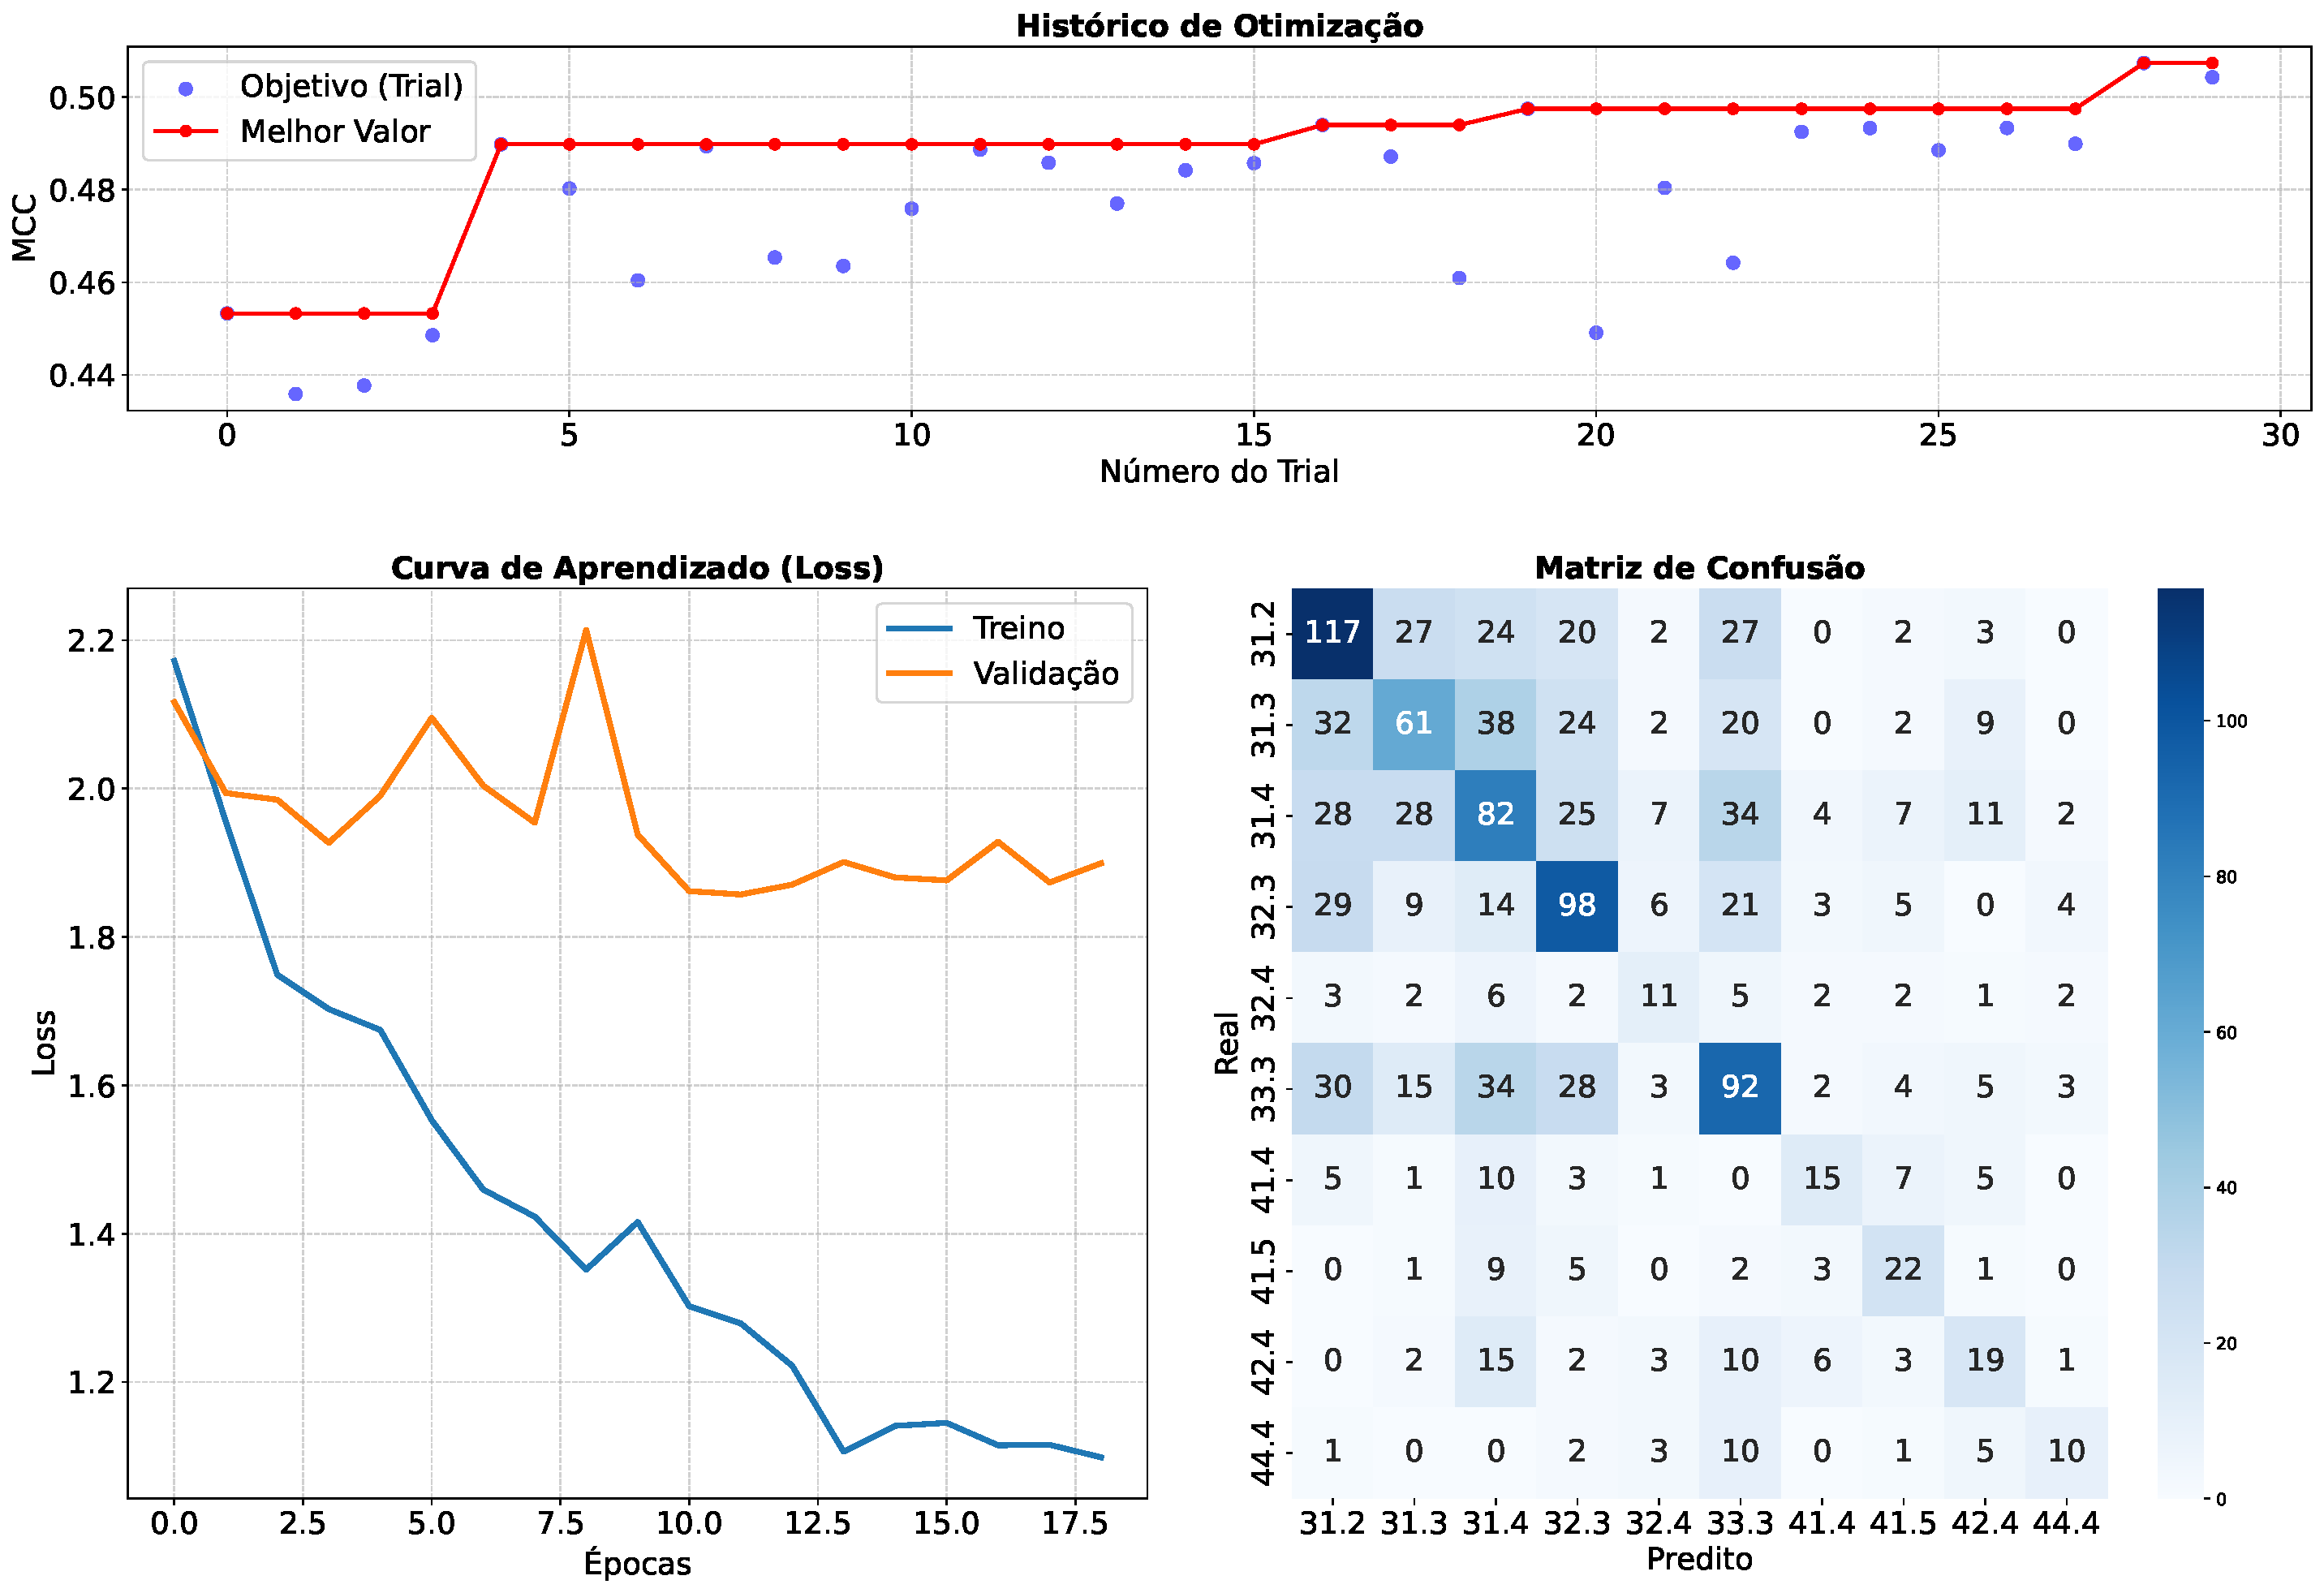
\includegraphics[width=0.85\textwidth]{tex/appendix/experiments/inception_v10_BR_opt_aug/dashboard_consolidado.pdf}
        \caption{Histórico de Otimização, Curvas de Aprendizado e Matriz de Confusão - inception\_v10\_BR\_opt\_aug}
    \end{figure}
\end{minipage}
\clearpage
